\chapter{Introduction}
\label{chp:introduction} 

\section{About the Project}

This thesis presents and documents this author's master's project, \textbf{TTK4900}, on robotic maintenance which was carried out at the Department of Engineering Cyberentics (ITK) in the spring of 2016. \textbf{TTK4900} is worth 30 credits (studiepoeng), and the project duration is set to 22 full-time weeks with the possibility of extension in case of a valid reason. The work presented in this thesis is carried out as independent work, which is supervised by Professor Tor Onshus through regular status meetings.

%\subsection{Long Term Goal and Previous Work}

\subsection{The Project Proposal - Mobile Autonomous Robot}

The robot system that was used in this project has been developed over the course of many preceding master and specialization projects. The long term goal of these projects is to develop mobile autonomous robot concepts for maintenance and inspection on topside offshore installations. The topic of this thesis is based on the project proposal which is given by Professor Tor Onshus at \ac{ITK}. A description of this proposal\footnote{\url{http://folk.ntnu.no/onshus/Oppgaver.htm}}, suggests some possible applications for such a robot: 

\begin{itemize}
	\item The robot could serve in a supporting role as a part of \ac{IO}.
	\item It can also be used to prepare a normally unmanned topside offshore installation before the arrival of a maintenance crew, by performing safety checks and preparing the helicopter landing pad.  
	\item Allow personnel to perform remote inspection and maintenance through telepresence.
	\item  In combination with \ac{VR}, the robot could be used for training purposes. 
\end{itemize}

\section{Preceding Projects}

\subsubsection{Telepresence and Robotic Arm}

The system in its current form is built around a robot manipulator arm, SCORBOT-ER4u. Kristian Saxrud Bekken focused on improving previous work on the system, which was done as early as 2005\cite{bekken}. Bekken's work comprise telepresence through a stereo video transmission, a collision avoidance system for the robot arm and an improved \ac{HMI} implementation.

\subsubsection{Building the Mobile Platform}
During the spring of 2013, Petter Aspunvik devoted his master's project to develop a mobile base for the robotic arm\cite{aspunvik}. Aspunvik's thesis has served as a user manual for many of the robot systems in the early stages of this project. The current motor control firmware used Aspunvik's implementation as a starting point.

\subsubsection{Simultaneous Localization and Mapping}

In parallel to Aspunvik's project, Mikael Berg developed a solution for \ac{SLAM} and autonomous navigation for the same robot\cite{berg}. His software is programmed in Google's Go language, and runs on Windows 7 within the pre-installed on-board computer. The resulting system successfully utilized Hector SLAM with a LIDAR and odometry from two encoder wheels for 2D navigation and \ac{SLAM}. Berg considered to create a solution based on \ac{ROS} which requires a Linux platform. In the end, he opted to target the Windows platform as this apparently is the only operating system which is compatible with the robotic arm. The ''future work''-section in Berg's thesis suggests improvements in the form of 3D obstruction detection, because the LIDAR is limited to detection in a plane. He also mentions object recognition and dynamic re-planning as possible extensions. 

\subsubsection{Last Year's Specialization Project}

This author's specialization project\cite{lindrup} presented an obstruction detector based on two unsynchronized IP-cameras and a stereo matching algorithm in \ac{OpenCV}. Because the cameras were unsynchronized, the system would become useless whenever there is relative motion between the robot and the surroundings. The obstruction detector lacked a critical feature: a floor filter to separate the ground from potential obstructions. The implementation presented in this master's project is unrelated to the preceding specialization project, except for some useful c++ functions and ideas that are brought forward.

\section{Implementation Overview}

\subsection{Deciding on a Goal}

To meet objective 4 in the problem description, it was decided to focus on vision based navigation. A robot with the ability to build a map of the surroundings and relocate autonomously was considered to be a good starting point for further development of vision based solutions.

\subsection{Selecting Tools and Hardware}

As a continuation of this author's specialization project, the robot was equipped with a 3D camera, a Kinect for XBOX 360 capable of perceiving depth images at a high frame rate ($30 Hz$). 

To use the Kinect, the initial plan was to utilize the \ac{PCL} in combination with a \ac{SLAM} method (e.g. Kintinous\cite{Kintinous}). This approach came with a high degree of uncertainty that would reduce the project scope significantly, and increase the likelihood of an unsatisfactory result. The Robot Operating System (ROS), an open source robot software framework, came up as an alternative tool late in January. 

The work and solutions presented in this thesis revolves around the process of integrating ROS with the mobile robot from \cite{aspunvik} and \cite{berg}. Installing ROS on Ubuntu Linux is by far the easiest way to begin using the framework. For this reason, and to avoid interfering with another project on the same robot, it was decided that an additional computer running Linux should be fitted to the robot. The mobile robot from \cite{aspunvik} and \cite{berg} was refitted to accommodate the Kinect and the second computer.

Two supporting tools were implemented in addition to the robot software: a simple concept of an \ac{OCS} and a hand held remote control implemented on a smartphone. An overview of the complete system is shown in figure \ref{fig:conseptDrawing}.

\begin{figure}[h]
	\centering
	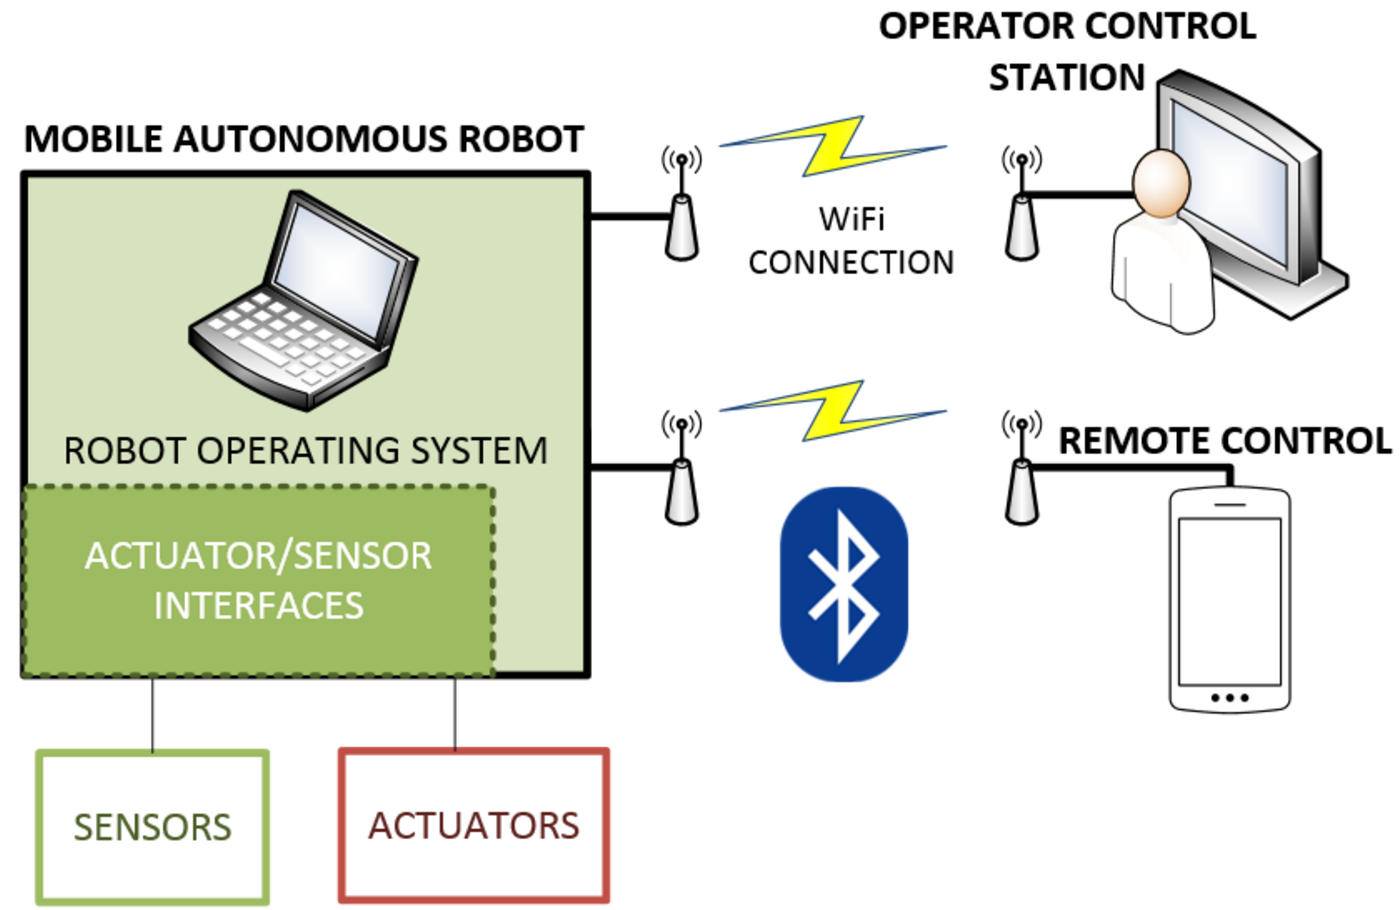
\includegraphics[width=0.8\textwidth]{conseptDrawing}
	\caption{System Concept. An on-board computer using \ac{ROS} to handle actuators and sensors. Remote operation is available through an \ac{OCS} or a hand-held device with Bluetooth.}
	\label{fig:conseptDrawing}
\end{figure}

\subsection{Functionality}

\begin{enumerate}
\item Simultaneous localization and mapping based on computer vision.
\item Mapping over multiple sessions.
\item Autonomous navigation to a simple goal.
\item 3D and 2D obstacle avoidance in navigation mode.
\item The robot can be controlled by an Android Smartphone.
\item The robot can stream video to an URL.
\item The robot can receive velocity commands over WiFi.
\end{enumerate} 

\section{Thesis Structure}

\subsubsection{Chapter \ref{chp:maintenance} - Robotic Maintenance on Topside Offshore Platforms} 

\subsubsection{Chapter \ref{chp:theory} - Background Theory}

\subsubsection{Chapter \ref{chp:implementation} - Implementation}

\subsubsection{Chapter \ref{chp:results} - Results}

\subsubsection{Chapter \ref{chp:discussion} - Discussion}

\subsubsection{Chapter \ref{chp:conclusion} - Conclusion}